%% bare_jrnl.tex
%% V1.4b
%% 2015/08/26
%% by Michael Shell
%% see http://www.michaelshell.org/
%% for current contact information.
%%
%% This is a skeleton file demonstrating the use of IEEEtran.cls
%% (requires IEEEtran.cls version 1.8b or later) with an IEEE
%% journal paper.
%%
%% Support sites:
%% http://www.michaelshell.org/tex/ieeetran/
%% http://www.ctan.org/pkg/ieeetran
%% and
%% http://www.ieee.org/

%%*************************************************************************
%% Legal Notice:
%% This code is offered as-is without any warranty either expressed or
%% implied; without even the implied warranty of MERCHANTABILITY or
%% FITNESS FOR A PARTICULAR PURPOSE! 
%% User assumes all risk.
%% In no event shall the IEEE or any contributor to this code be liable for
%% any damages or losses, including, but not limited to, incidental,
%% consequential, or any other damages, resulting from the use or misuse
%% of any information contained here.
%%
%% All comments are the opinions of their respective authors and are not
%% necessarily endorsed by the IEEE.
%%
%% This work is distributed under the LaTeX Project Public License (LPPL)
%% ( http://www.latex-project.org/ ) version 1.3, and may be freely used,
%% distributed and modified. A copy of the LPPL, version 1.3, is included
%% in the base LaTeX documentation of all distributions of LaTeX released
%% 2003/12/01 or later.
%% Retain all contribution notices and credits.
%% ** Modified files should be clearly indicated as such, including  **
%% ** renaming them and changing author support contact information. **
%%*************************************************************************


% *** Authors should verify (and, if needed, correct) their LaTeX system  ***
% *** with the testflow diagnostic prior to trusting their LaTeX platform ***
% *** with production work. The IEEE's font choices and paper sizes can   ***
% *** trigger bugs that do not appear when using other class files.       ***                          ***
% The testflow support page is at:
% http://www.michaelshell.org/tex/testflow/



\documentclass[journal]{IEEEtran}
%
% If IEEEtran.cls has not been installed into the LaTeX system files,
% manually specify the path to it like:
% \documentclass[journal]{../sty/IEEEtran}





% Some very useful LaTeX packages include:
% (uncomment the ones you want to load)


% *** MISC UTILITY PACKAGES ***
%
%\usepackage{ifpdf}
% Heiko Oberdiek's ifpdf.sty is very useful if you need conditional
% compilation based on whether the output is pdf or dvi.
% usage:
% \ifpdf
%   % pdf code
% \else
%   % dvi code
% \fi
% The latest version of ifpdf.sty can be obtained from:
% http://www.ctan.org/pkg/ifpdf
% Also, note that IEEEtran.cls V1.7 and later provides a builtin
% \ifCLASSINFOpdf conditional that works the same way.
% When switching from latex to pdflatex and vice-versa, the compiler may
% have to be run twice to clear warning/error messages.






% *** CITATION PACKAGES ***
%
%\usepackage{cite}
% cite.sty was written by Donald Arseneau
% V1.6 and later of IEEEtran pre-defines the format of the cite.sty package
% \cite{} output to follow that of the IEEE. Loading the cite package will
% result in citation numbers being automatically sorted and properly
% "compressed/ranged". e.g., [1], [9], [2], [7], [5], [6] without using
% cite.sty will become [1], [2], [5]--[7], [9] using cite.sty. cite.sty's
% \cite will automatically add leading space, if needed. Use cite.sty's
% noadjust option (cite.sty V3.8 and later) if you want to turn this off
% such as if a citation ever needs to be enclosed in parenthesis.
% cite.sty is already installed on most LaTeX systems. Be sure and use
% version 5.0 (2009-03-20) and later if using hyperref.sty.
% The latest version can be obtained at:
% http://www.ctan.org/pkg/cite
% The documentation is contained in the cite.sty file itself.






% *** GRAPHICS RELATED PACKAGES ***
%
\ifCLASSINFOpdf
  % \usepackage[pdftex]{graphicx}
  % declare the path(s) where your graphic files are
  % \graphicspath{{../pdf/}{../jpeg/}}
  % and their extensions so you won't have to specify these with
  % every instance of \includegraphics
  % \DeclareGraphicsExtensions{.pdf,.jpeg,.png}
\else
  % or other class option (dvipsone, dvipdf, if not using dvips). graphicx
  % will default to the driver specified in the system graphics.cfg if no
  % driver is specified.
  % \usepackage[dvips]{graphicx}
  % declare the path(s) where your graphic files are
  % \graphicspath{{../eps/}}
  % and their extensions so you won't have to specify these with
  % every instance of \includegraphics
  % \DeclareGraphicsExtensions{.eps}
\fi
% graphicx was written by David Carlisle and Sebastian Rahtz. It is
% required if you want graphics, photos, etc. graphicx.sty is already
% installed on most LaTeX systems. The latest version and documentation
% can be obtained at: 
% http://www.ctan.org/pkg/graphicx
% Another good source of documentation is "Using Imported Graphics in
% LaTeX2e" by Keith Reckdahl which can be found at:
% http://www.ctan.org/pkg/epslatex
%
% latex, and pdflatex in dvi mode, support graphics in encapsulated
% postscript (.eps) format. pdflatex in pdf mode supports graphics
% in .pdf, .jpeg, .png and .mps (metapost) formats. Users should ensure
% that all non-photo figures use a vector format (.eps, .pdf, .mps) and
% not a bitmapped formats (.jpeg, .png). The IEEE frowns on bitmapped formats
% which can result in "jaggedy"/blurry rendering of lines and letters as
% well as large increases in file sizes.
%
% You can find documentation about the pdfTeX application at:
% http://www.tug.org/applications/pdftex





% *** MATH PACKAGES ***
%
%\usepackage{amsmath}
% A popular package from the American Mathematical Society that provides
% many useful and powerful commands for dealing with mathematics.
%
% Note that the amsmath package sets \interdisplaylinepenalty to 10000
% thus preventing page breaks from occurring within multiline equations. Use:
%\interdisplaylinepenalty=2500
% after loading amsmath to restore such page breaks as IEEEtran.cls normally
% does. amsmath.sty is already installed on most LaTeX systems. The latest
% version and documentation can be obtained at:
% http://www.ctan.org/pkg/amsmath





% *** SPECIALIZED LIST PACKAGES ***
%
%\usepackage{algorithmic}
% algorithmic.sty was written by Peter Williams and Rogerio Brito.
% This package provides an algorithmic environment fo describing algorithms.
% You can use the algorithmic environment in-text or within a figure
% environment to provide for a floating algorithm. Do NOT use the algorithm
% floating environment provided by algorithm.sty (by the same authors) or
% algorithm2e.sty (by Christophe Fiorio) as the IEEE does not use dedicated
% algorithm float types and packages that provide these will not provide
% correct IEEE style captions. The latest version and documentation of
% algorithmic.sty can be obtained at:
% http://www.ctan.org/pkg/algorithms
% Also of interest may be the (relatively newer and more customizable)
% algorithmicx.sty package by Szasz Janos:
% http://www.ctan.org/pkg/algorithmicx




% *** ALIGNMENT PACKAGES ***
%
%\usepackage{array}
% Frank Mittelbach's and David Carlisle's array.sty patches and improves
% the standard LaTeX2e array and tabular environments to provide better
% appearance and additional user controls. As the default LaTeX2e table
% generation code is lacking to the point of almost being broken with
% respect to the quality of the end results, all users are strongly
% advised to use an enhanced (at the very least that provided by array.sty)
% set of table tools. array.sty is already installed on most systems. The
% latest version and documentation can be obtained at:
% http://www.ctan.org/pkg/array


% IEEEtran contains the IEEEeqnarray family of commands that can be used to
% generate multiline equations as well as matrices, tables, etc., of high
% quality.




% *** SUBFIGURE PACKAGES ***
%\ifCLASSOPTIONcompsoc
%  \usepackage[caption=false,font=normalsize,labelfont=sf,textfont=sf]{subfig}
%\else
%  \usepackage[caption=false,font=footnotesize]{subfig}
%\fi
% subfig.sty, written by Steven Douglas Cochran, is the modern replacement
% for subfigure.sty, the latter of which is no longer maintained and is
% incompatible with some LaTeX packages including fixltx2e. However,
% subfig.sty requires and automatically loads Axel Sommerfeldt's caption.sty
% which will override IEEEtran.cls' handling of captions and this will result
% in non-IEEE style figure/table captions. To prevent this problem, be sure
% and invoke subfig.sty's "caption=false" package option (available since
% subfig.sty version 1.3, 2005/06/28) as this is will preserve IEEEtran.cls
% handling of captions.
% Note that the Computer Society format requires a larger sans serif font
% than the serif footnote size font used in traditional IEEE formatting
% and thus the need to invoke different subfig.sty package options depending
% on whether compsoc mode has been enabled.
%
% The latest version and documentation of subfig.sty can be obtained at:
% http://www.ctan.org/pkg/subfig




% *** FLOAT PACKAGES ***
%
%\usepackage{fixltx2e}
% fixltx2e, the successor to the earlier fix2col.sty, was written by
% Frank Mittelbach and David Carlisle. This package corrects a few problems
% in the LaTeX2e kernel, the most notable of which is that in current
% LaTeX2e releases, the ordering of single and double column floats is not
% guaranteed to be preserved. Thus, an unpatched LaTeX2e can allow a
% single column figure to be placed prior to an earlier double column
% figure.
% Be aware that LaTeX2e kernels dated 2015 and later have fixltx2e.sty's
% corrections already built into the system in which case a warning will
% be issued if an attempt is made to load fixltx2e.sty as it is no longer
% needed.
% The latest version and documentation can be found at:
% http://www.ctan.org/pkg/fixltx2e


%\usepackage{stfloats}
% stfloats.sty was written by Sigitas Tolusis. This package gives LaTeX2e
% the ability to do double column floats at the bottom of the page as well
% as the top. (e.g., "\begin{figure*}[!b]" is not normally possible in
% LaTeX2e). It also provides a command:
%\fnbelowfloat
% to enable the placement of footnotes below bottom floats (the standard
% LaTeX2e kernel puts them above bottom floats). This is an invasive package
% which rewrites many portions of the LaTeX2e float routines. It may not work
% with other packages that modify the LaTeX2e float routines. The latest
% version and documentation can be obtained at:
% http://www.ctan.org/pkg/stfloats
% Do not use the stfloats baselinefloat ability as the IEEE does not allow
% \baselineskip to stretch. Authors submitting work to the IEEE should note
% that the IEEE rarely uses double column equations and that authors should try
% to avoid such use. Do not be tempted to use the cuted.sty or midfloat.sty
% packages (also by Sigitas Tolusis) as the IEEE does not format its papers in
% such ways.
% Do not attempt to use stfloats with fixltx2e as they are incompatible.
% Instead, use Morten Hogholm'a dblfloatfix which combines the features
% of both fixltx2e and stfloats:
%
% \usepackage{dblfloatfix}
% The latest version can be found at:
% http://www.ctan.org/pkg/dblfloatfix




%\ifCLASSOPTIONcaptionsoff
%  \usepackage[nomarkers]{endfloat}
% \let\MYoriglatexcaption\caption
% \renewcommand{\caption}[2][\relax]{\MYoriglatexcaption[#2]{#2}}
%\fi
% endfloat.sty was written by James Darrell McCauley, Jeff Goldberg and 
% Axel Sommerfeldt. This package may be useful when used in conjunction with 
% IEEEtran.cls'  captionsoff option. Some IEEE journals/societies require that
% submissions have lists of figures/tables at the end of the paper and that
% figures/tables without any captions are placed on a page by themselves at
% the end of the document. If needed, the draftcls IEEEtran class option or
% \CLASSINPUTbaselinestretch interface can be used to increase the line
% spacing as well. Be sure and use the nomarkers option of endfloat to
% prevent endfloat from "marking" where the figures would have been placed
% in the text. The two hack lines of code above are a slight modification of
% that suggested by in the endfloat docs (section 8.4.1) to ensure that
% the full captions always appear in the list of figures/tables - even if
% the user used the short optional argument of \caption[]{}.
% IEEE papers do not typically make use of \caption[]'s optional argument,
% so this should not be an issue. A similar trick can be used to disable
% captions of packages such as subfig.sty that lack options to turn off
% the subcaptions:
% For subfig.sty:
% \let\MYorigsubfloat\subfloat
% \renewcommand{\subfloat}[2][\relax]{\MYorigsubfloat[]{#2}}
% However, the above trick will not work if both optional arguments of
% the \subfloat command are used. Furthermore, there needs to be a
% description of each subfigure *somewhere* and endfloat does not add
% subfigure captions to its list of figures. Thus, the best approach is to
% avoid the use of subfigure captions (many IEEE journals avoid them anyway)
% and instead reference/explain all the subfigures within the main caption.
% The latest version of endfloat.sty and its documentation can obtained at:
% http://www.ctan.org/pkg/endfloat
%
% The IEEEtran \ifCLASSOPTIONcaptionsoff conditional can also be used
% later in the document, say, to conditionally put the References on a 
% page by themselves.




% *** PDF, URL AND HYPERLINK PACKAGES ***
%
%\usepackage{url}
% url.sty was written by Donald Arseneau. It provides better support for
% handling and breaking URLs. url.sty is already installed on most LaTeX
% systems. The latest version and documentation can be obtained at:
% http://www.ctan.org/pkg/url
% Basically, \url{my_url_here}.




% *** Do not adjust lengths that control margins, column widths, etc. ***
% *** Do not use packages that alter fonts (such as pslatex).         ***
% There should be no need to do such things with IEEEtran.cls V1.6 and later.
% (Unless specifically asked to do so by the journal or conference you plan
% to submit to, of course. )


% correct bad hyphenation here
\hyphenation{op-tical net-works semi-conduc-tor}
\usepackage{array}
\usepackage{graphicx}

\begin{document}
%
% paper title
% Titles are generally capitalized except for words such as a, an, and, as,
% at, but, by, for, in, nor, of, on, or, the, to and up, which are usually
% not capitalized unless they are the first or last word of the title.
% Linebreaks \\ can be used within to get better formatting as desired.
% Do not put math or special symbols in the title.
\title{The Role of Cybersecurity in Information Systems in Organizations: a systematic literature review}
%
%
% author names and IEEE memberships
% note positions of commas and nonbreaking spaces ( ~ ) LaTeX will not break
% a structure at a ~ so this keeps an author's name from being broken across
% two lines.
% use \thanks{} to gain access to the first footnote area
% a separate \thanks must be used for each paragraph as LaTeX2e's \thanks
% was not built to handle multiple paragraphs
%

%\author{Eduardo~Santos
%        John~Doe,~\IEEEmembership{Fellow,~OSA,}
%        and~Jane~Doe,~\IEEEmembership{Life~Fellow,~IEEE}

\author{Eduardo~Santos,
        Gonçalo~Passos,
        Pedro~Bastos,
        and~Pedro~Sobral,~DETI UA% <-this % stops a space
}

% note the % following the last \IEEEmembership and also \thanks - 
% these prevent an unwanted space from occurring between the last author name
% and the end of the author line. i.e., if you had this:
% 
% \author{....lastname \thanks{...} \thanks{...} }
%                     ^------------^------------^----Do not want these spaces!
%
% a space would be appended to the last name and could cause every name on that
% line to be shifted left slightly. This is one of those "LaTeX things". For
% instance, "\textbf{A} \textbf{B}" will typeset as "A B" not "AB". To get
% "AB" then you have to do: "\textbf{A}\textbf{B}"
% \thanks is no different in this regard, so shield the last } of each \thanks
% that ends a line with a % and do not let a space in before the next \thanks.
% Spaces after \IEEEmembership other than the last one are OK (and needed) as
% you are supposed to have spaces between the names. For what it is worth,
% this is a minor point as most people would not even notice if the said evil
% space somehow managed to creep in.



% The paper headers
%\markboth{Journal of \LaTeX\ Class Files,~Vol.~14, No.~8, %August~2015}%
%{Shell \MakeLowercase{\textit{et al.}}: Bare Demo of %IEEEtran.cls for IEEE Journals}
% The only time the second header will appear is for the odd numbered pages
% after the title page when using the twoside option.
% 
% *** Note that you probably will NOT want to include the author's ***
% *** name in the headers of peer review papers.                   ***
% You can use \ifCLASSOPTIONpeerreview for conditional compilation here if
% you desire.




% If you want to put a publisher's ID mark on the page you can do it like
% this:
%\IEEEpubid{0000--0000/00\$00.00~\copyright~2015 IEEE}
% Remember, if you use this you must call \IEEEpubidadjcol in the second
% column for its text to clear the IEEEpubid mark.



% use for special paper notices
%\IEEEspecialpapernotice{(Invited Paper)}




% make the title area
\maketitle

%Abstract
%Purpose – This paper aims to conduct a review of the literature published, between %2006 and 2018, that used search engine data on tourism and hospitality research, %namely, Google Insights for Search and Google Trends. More specifically, it intends %to identify the purpose and context of the data use, ascertaining the main findings %and reviewing the methodological approaches.
%Design/methodology/approach – A systematic literature review of Scopus indexed %research has been carried out. Given the novelty of search engine data use in tourism %and hospitality research and the relatively low number of search results in Scopus, %other databases were used to broaden the scope of analysis, namely, EBSCO and Google %Scholar. The papers selected were subjected to content and statistical analyses.
%Findings – Google Trends data use in tourism and hospitality research has increased %significantly from 2012 to 2017, mainly for tourism forecasting/nowcasting; knowing %the interest of users’ searches for tourist attractions or destinations; showing the %relationship between the official tourism statistics and the search volume index of %Google Trends; and estimating the effect of one event on tourism demand. The %categories and search terms used vary with the purpose of the study; however, they %mostly focus on the travel category and use the country as the search term.
%Originality/value – Google Trends has been increasingly used in research publications %in tourism and hospitality, but the range of its applications and methods used has %not yet been reviewed. Therefore, a systematic review of the existing literature %increases awareness of its potential uses in tourism and hospitality research and %facilitates a better understanding of its strengths and weaknesses as a research tool.
%Keywords GoogleTrends,Tourismandhospitality,Systematicreview,Searchenginedata, Google %insights for search
%Paper type Literature review

% As a general rule, do not put math, special symbols or citations
% in the abstract or keywords.
\begin{abstract}
This paper presents a systematic literature review examining the role of cybersecurity in information systems in organizations. The review presents an in-depth analysis of ten studies published between 2017 and 2023 and aims to identify the significance and role of cybersecurity in information systems within organizations. This systematic review was carried out from relevant research using the Scopus database.

The analysed documents reveal an increasing trend in cyber-attacks, attributing this rise to the growing permeability of organizational boundaries in the digital age. They underscore the importance of robust systems, such as Supervisory Control and Data Acquisition (SCADA), in maintaining real-time control and monitoring of critical infrastructures.

The review also highlights the critical role of cybersecurity awareness within organizations. It emphasizes the need for a strong security culture, underpinned by continuous education and training, to enhance the overall resilience of organizations against cyber threats.

The rapid pace of digital modernization and its implications for cybersecurity is another key theme. The documents point to the escalating complexity of cybersecurity threats in the wake of digital transformation and stress the importance of regular security audits in managing these risks effectively.

The role of top management and their influence on cybersecurity practices is also explored. The documents suggest that those in the highest positions, including the Chief Information Officer (CIO), should take a proactive role in integrating cybersecurity into the broader business strategy.

In conclusion, this review provides a comprehensive understanding of the multifaceted role of cybersecurity in information systems within organizations. It also identifies potential avenues for future research, emphasizing the need for empirical investigations, exploration of cultural influences, and case studies focusing on security success outcomes.
\end{abstract}

% Note that keywords are not normally used for peerreview papers.
\begin{IEEEkeywords}
Cybersecurity, Information Systems, Security Of Data, \LaTeX, Security Systems, Data Privacy.
\end{IEEEkeywords}






% For peer review papers, you can put extra information on the cover
% page as needed:
% \ifCLASSOPTIONpeerreview
% \begin{center} \bfseries EDICS Category: 3-BBND \end{center}
% \fi
%
% For peerreview papers, this IEEEtran command inserts a page break and
% creates the second title. It will be ignored for other modes.
\IEEEpeerreviewmaketitle


\section{Introduction}

% The very first letter is a 2 line initial drop letter followed
% by the rest of the first word in caps.
% 
% form to use if the first word consists of a single letter:
% \IEEEPARstart{A}{demo} file is ....
% 
% form to use if you need the single drop letter followed by
% normal text (unknown if ever used by the IEEE):
% \IEEEPARstart{A}{}demo file is ....
% 
% Some journals put the first two words in caps:
% \IEEEPARstart{T}{his demo} file is ....
% 
% Here we have the typical use of a "T" for an initial drop letter
% and "HIS" in caps to complete the first word.
\IEEEPARstart{C}{ybersecurity} has become a major concern for businesses all over the world in the modern digital era. The potential for cyber threats has exploded as digital technologies continue to develop and permeate every aspect of organizational operations. The security and integrity of information systems within organizations are seriously at risk from these threats, which include data breaches and sophisticated cyberattacks.

The cybersecurity landscape has changed significantly over the last few years. New opportunities for efficiency and innovation have been created by the emergence of technologies like cloud computing, AI, and the Internet of Things (IoT). The task of securing information systems has become more difficult as a result of the new vulnerabilities and attack vectors that have been brought about by these developments.

The nature of cyber threats has also changed, in addition to technological advancements. Cybercriminals are becoming more skilled, using cutting-edge methods, and continuously modifying security precautions. The cybersecurity environment has become even more complicated as a result of state-sponsored cyberattacks and cyberespionage.

Additionally, the challenges associated with cybersecurity have been exacerbated by the rise of remote work in response to the global pandemic. In order to quickly adapt to a distributed workforce, organizations frequently lacked the necessary security infrastructure, making them more susceptible to cyber-attacks.

Understanding the function of cybersecurity in information systems in this context is crucial for organizations on a strategic level. It requires a comprehensive strategy that takes organizational culture, human factors, and strategic considerations into account in addition to technological measures.

Using the most recent findings and advancements in the field, this paper aims to present a thorough overview of the current state of cybersecurity in information systems within organizations. It will go into depth on important subjects like the causes of the rise in cyberattacks, the value of cybersecurity awareness within organizations, the effects of digital modernization on cybersecurity, and the responsibility of top management in preventing and managing security breaches.

The importance of cybersecurity in information systems will undoubtedly continue to develop as we move through the digital transformation era, demanding ongoing research, vigilance, and adaptation.


\section{Methodology}

In this study, a systematic literature review is conducted to obtain a comprehensive understanding of the current state-of-the-art regarding the role of Cybersecurity in Information Systems in Organizations. The primary goal of this review is to evaluate the published articles in this field and gain insights into the studies' objectives, data collection and analysis methods carried out, as well as the key findings.
This section provides a detailed account of the methodology employed in conducting the literature review, including article selection and analysis processes, and presents the thematic areas covered by the selected articles.

\subsection{Selection of the articles}

The Scopus database was used to search and find the publications intended for this review. The query ("cybersecurity" AND "role" AND "Information Systems" AND "Organizations") with the time period between 2017 and 2023 returned 29 documents, where 10 were excluded for not being within the scope of this literature review. The abstract and introduction of the 19 articles were closely analysed and we concluded that 9 of them had a small substantial matter for this study case and were eliminated. 
With that in mind, 10 articles were determined relevant and included in this literature review. This process is presented in Figure \ref{articles}.


\begin{figure}[!h]
    \centering
    \caption{Article selection process}
    \label{articles}
    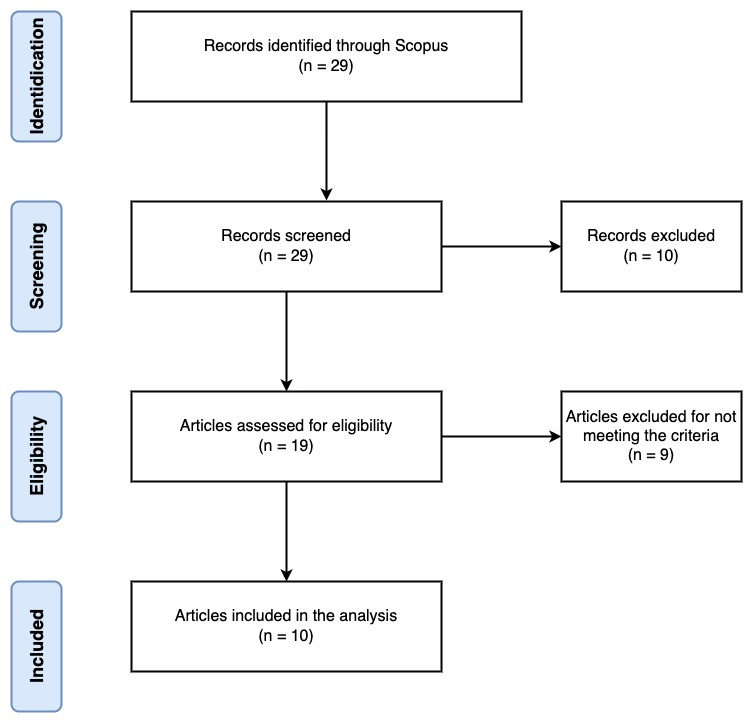
\includegraphics[width=\linewidth]{images/articles.jpg}
\end{figure}


\subsection{Data analysis}

To successfully understand each article and how they can correlate with each other, we were able to group them into 4 main topics (Table \ref{table_1}).

\begin{table}[h!]
    \renewcommand{\arraystretch}{1.3}
    \normalsize
    \caption{Topics and Articles}
    \label{table_1}
    \centering
    
    \begin{tabular}{ m{18em} m{5em} }
        \hline
        \textbf{Topics} & \textbf{Publications} \\
        \hline
        \textit{Cyber Security Awareness in Organizations} & \cite{Steps_article1}, \cite{Edu_article1} \\
        \hline
        \textit{Reasons for Increase in Cyber-attacks}   & \cite{Edu_article4}\cite{sobral_1}, \cite{sobral_2} \\
        \hline
        \textit{Importance of the Highest Positions in the Prevention and Management of Security Breaches} & \cite{Steps_article3}, \cite{article3}, \cite{article11} \\
        \hline
        \textit{The Role of External Auditors and IT Modernization in Reducing Cybersecurity Risks} & \cite{bastos_1}, \cite{bastos_2} \\
        \hline
    \end{tabular}
    
\end{table}

\subsection{Article analysis}

The interest in the cybersecurity within the organizations is growing at a faster rate than ever. More and more organizations have been spending effort, time and money into this field and its growth reflects on the investigation carried in it. For that reason, the best and most relevant articles found in this area are from the last 4-5 years. Figure \ref{years} shows the distribution of the included articles in each year.

\begin{figure}[!h]
    \centering
    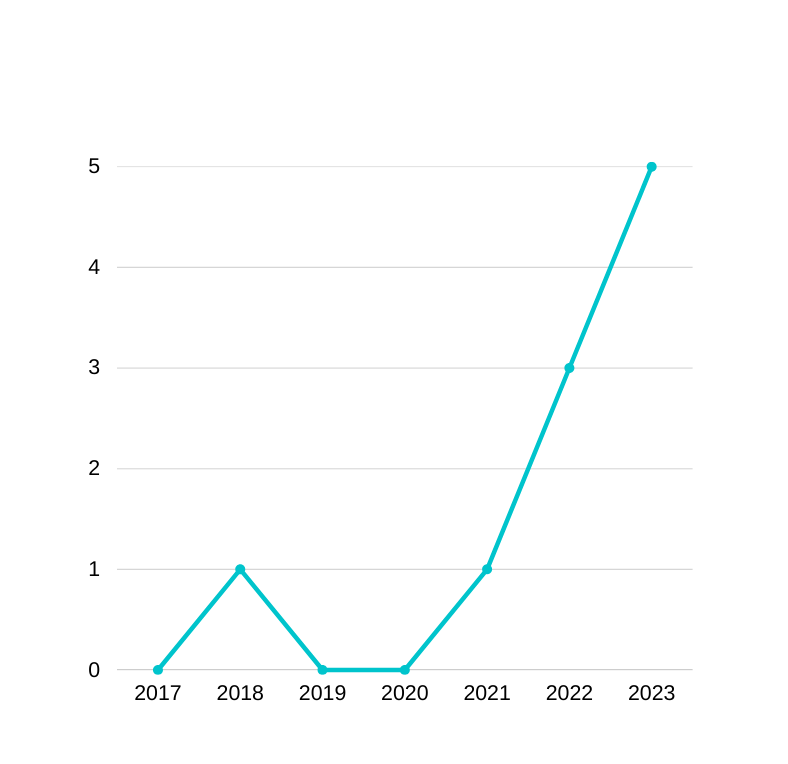
\includegraphics[width=\linewidth]{images/years.png}
    \caption{Article distribution}
    \label{years}
\end{figure}



\section{Cyber Security Awareness in Organizations}

In the modern era, the Internet has become a staple for a multitude of activities, including e-commerce and online banking. As a result, cybersecurity has emerged as a critical issue, particularly for the financial sector, which is frequently targeted by cyber threats \cite{Edu_article1}, although many other sectors suffer from this problem. 

These dangers can manifest in a variety of ways, such as email phishing, ransomware, malware, and denial-of-service (DoS) attacks, etc., and they have a wide range of effects on organizations. However, if users are aware of cybersecurity issues, the risks posed by these threats can be reduced. According to the Information Security Awareness (ISA) model, a number of personal factors, such as cybersecurity training, educational background, work experience, field of study, gender, age, training, and place of residence, have an impact on this awareness \cite{Edu_article1}. 

In order to protect users' assets and the environment of the organization, cybersecurity encompasses a range of best practices, concepts, policies, assurances, guidelines, safeguards, actions, risk management strategies, training, tools, and technologies. Any information found in the cyber environment, including networked devices, infrastructure, telecommunications systems, services, and applications, can be included in these assets. They must be protected based on the CIA's three main goals of confidentiality (C), integrity (I), and availability (A).

Understanding security threats and taking the necessary precautions to reduce risks is known as cybersecurity awareness (CSA). It is essential to give CSA training to people who work directly with information systems. This instruction can improve both the organization's and the individuals' level of protection.

It is argued that developing an information security culture will lead to a secure organization. Members of the organization act as its first line of defense in this situation. Employees frequently fall victim to social engineering techniques employed by hackers, or they act carelessly endangering the security of crucial information assets within an organization \cite{Steps_article2}.

In addition to cybersecurity, information security involves data protection measures, such as the General Data Protection Regulation (GDPR), which safeguard sensitive data from unauthorized access, exposure, or theft.

A number of demographic factors, such as gender, age, nationality, field of study, work experience, and training, affect cybersecurity awareness. For instance, it's been discovered that gender can influence security self-efficacy, prior experience, and computer skills. It's also been discovered that years of computer usage or experience, as well as gender, significantly influence the rate of phishing detection \cite{Edu_article1}.




% An example of a floating figure using the graphicx package.
% Note that \label must occur AFTER (or within) \caption.
% For figures, \caption should occur after the \includegraphics.
% Note that IEEEtran v1.7 and later has special internal code that
% is designed to preserve the operation of \label within \caption
% even when the captionsoff option is in effect. However, because
% of issues like this, it may be the safest practice to put all your
% \label just after \caption rather than within \caption{}.
%
% Reminder: the "draftcls" or "draftclsnofoot", not "draft", class
% option should be used if it is desired that the figures are to be
% displayed while in draft mode.
%
%\begin{figure}[!t]
%\centering
%\includegraphics[width=2.5in]{myfigure}
% where an .eps filename suffix will be assumed under latex, 
% and a .pdf suffix will be assumed for pdflatex; or what has been declared
% via \DeclareGraphicsExtensions.
%\caption{Simulation results for the network.}
%\label{fig_sim}
%\end{figure}

% Note that the IEEE typically puts floats only at the top, even when this
% results in a large percentage of a column being occupied by floats.


% An example of a double column floating figure using two subfigures.
% (The subfig.sty package must be loaded for this to work.)
% The subfigure \label commands are set within each subfloat command,
% and the \label for the overall figure must come after \caption.
% \hfil is used as a separator to get equal spacing.
% Watch out that the combined width of all the subfigures on a 
% line do not exceed the text width or a line break will occur.
%
%\begin{figure*}[!t]
%\centering
%\subfloat[Case I]{\includegraphics[width=2.5in]{box}%
%\label{fig_first_case}}
%\hfil
%\subfloat[Case II]{\includegraphics[width=2.5in]{box}%
%\label{fig_second_case}}
%\caption{Simulation results for the network.}
%\label{fig_sim}
%\end{figure*}
%
% Note that often IEEE papers with subfigures do not employ subfigure
% captions (using the optional argument to \subfloat[]), but instead will
% reference/describe all of them (a), (b), etc., within the main caption.
% Be aware that for subfig.sty to generate the (a), (b), etc., subfigure
% labels, the optional argument to \subfloat must be present. If a
% subcaption is not desired, just leave its contents blank,
% e.g., \subfloat[].


% An example of a floating table. Note that, for IEEE style tables, the
% \caption command should come BEFORE the table and, given that table
% captions serve much like titles, are usually capitalized except for words
% such as a, an, and, as, at, but, by, for, in, nor, of, on, or, the, to
% and up, which are usually not capitalized unless they are the first or
% last word of the caption. Table text will default to \footnotesize as
% the IEEE normally uses this smaller font for tables.
% The \label must come after \caption as always.
%
%\begin{table}[!t]
%% increase table row spacing, adjust to taste
%\renewcommand{\arraystretch}{1.3}
% if using array.sty, it might be a good idea to tweak the value of
% \extrarowheight as needed to properly center the text within the cells
%\caption{An Example of a Table}
%\label{table_example}
%\centering
%% Some packages, such as MDW tools, offer better commands for making tables
%% than the plain LaTeX2e tabular which is used here.
%\begin{tabular}{|c||c|}
%\hline
%One & Two\\
%\hline
%Three & Four\\
%\hline
%\end{tabular}
%\end{table}


% Note that the IEEE does not put floats in the very first column
% - or typically anywhere on the first page for that matter. Also,
% in-text middle ("here") positioning is typically not used, but it
% is allowed and encouraged for Computer Society conferences (but
% not Computer Society journals). Most IEEE journals/conferences use
% top floats exclusively. 
% Note that, LaTeX2e, unlike IEEE journals/conferences, places
% footnotes above bottom floats. This can be corrected via the
% \fnbelowfloat command of the stfloats package.


\section{Reasons for Increase in Cyber-attacks}

Cyber attacks are increasingly being talked about, and the consequences of these attacks are being recognized as extremely harmful. Every day, more and more devices are being connected to the Internet, and this trend is visible across various sectors of the industry and essential services.
The increasing digitization of systems and services in areas like health information systems, Industrial Internet of Things, and remote work creates new cyberattack surfaces requiring robust and evolving cybersecurity measures, from all the actors. The main rule/concept to reduce cybercrime in all these sectors goes through  developing comprehensive cybersecurity policies and implementing both basic and advanced security controls. 

Healthcare organizations needs a lot of security in the virtual layer, the concept of privacy in this sector is a main character, and is very important to have the right security policies to protect the sensitive user data. 
It is important to emphasize the regular compliance checks with security standards, in order to understand the latest regulations that must be applied in health information systems, in order to reduce (at least try) the vulnerabilities.
The greatest vulnerability in healthcare organizations is the human factor, emphasizing the need for more support for healthcare cybersecurity professionals and their cybersecurity programs \cite{Edu_article3}.

In the context of the Industrial Internet of Things (IIoT), sectors such as transport, energy, and industry face unique security threats. The integration of new internet-connected devices into critical infrastructure operations is creating new attack surfaces that can expose critical functionalities to cyberattacks with severe consequences. Given all these attacks, new technologies and cybersecurity methods will be necessary to address the challenging technical aspect of operating IIoT equipment securely.
 A critical insight is the potential for systemic risk, where a security breach in one part of the IIoT can potentially affect other parts of the system, causing widespread disruptions or even physical damage \cite{sobral_1}.

As the number of end-users (largely remote workers) connecting remotely to a server or network increased very significantly in the last years, so more people are exposed to cyberattacks every day and the attack surface inevitably expands. Some of the best practices for remote work are: the use of various communication channels, regular training sessions on cybersecurity awareness, and the use of technological solutions such as endpoint security software like VPNs and firewalls. Other good practices to maintain cybersecurity awareness are: having strong and unique passwords, keeping the software and operating systems updated, being wary of phishing emails and suspicious links, and avoiding the use of public Wi-Fi for work-related activities \cite{sobral_2}.

In our increasingly interconnected world, the constant influx of devices connecting to the internet has resulted in a higher number of vulnerabilities within networks. The primary objective remains addressing existing vulnerabilities and providing knowledge on mitigating potential risks. The three topics mentioned above emphasize the necessity of a comprehensive cybersecurity approach across all sectors and modes of operation, emphasizing the importance of robust and adaptable security policies. This approach recognizes the ever-changing nature of cybersecurity threats and the need to continually update defenses. By prioritizing comprehensive training and awareness programs, individuals can acquire the skills needed to identify and respond to emerging cyber threats effectively. Moreover, the integration of advanced technological solutions is essential for proactive threat detection and neutralization. By adopting this comprehensive approach, we can create a safer digital environment, protecting critical information and infrastructure in our interconnected world.



\section{Importance of the Highest Positions in the Prevention and Management of Security Breaches}

An essential component of cybersecurity governance is the significance of the top positions inside businesses, especially top management teams (TMTs), in the prevention and management of security breaches. 

It is important to have information security risk assessments (ISRAs) in the wake of cybersecurity breaches, as is the mediating function of TMT attention to cybersecurity, as introduced by \cite{article3} . It emphasizes how robust responses to violations must take into account both internal and external factors. The cost of a breach affects the TMT's attention to cybersecurity, and higher breach costs cause more attention to be paid to security because of the failure to ensure security and the obligation to stakeholders. The study emphasizes the connection between breach costs, TMT security awareness, and the choice to do an ISRA. The findings highlight the significance of TMTs in setting cybersecurity as a top priority and devoting funds for risk analysis and management.

\cite{article11} takes a strategic leadership stance and focuses on digital firms' cyber-resiliency. It draws attention to the negative effects of cyberattacks on reputation, data loss, and knowledge loss. The paper stresses how little is known empirically about how strategic leaders influence and support cybersecurity strategies. The study outlines recommended practices for achieving cyber-resiliency through exploratory interviews with Chief Information Officers (CIOs), Chief Security Information Officers (CSIOs), and Chief Technology Officers (CTOs). Making cyber-resilience a crucial organizational competency, comprehending the ecosystem and interactions with partners and suppliers, developing governance frameworks, and allocating responsibility for the success of cybersecurity strategies are some examples of these techniques. The conclusions of this article emphasize the critical part that strategic leaders play in promoting cybersecurity measures and incorporating them into business culture.

As emphasized by \cite{Steps_article3}, it is important to build formal leadership development programs that are specifically designed for cybersecurity and information technology (IT) professionals. It emphasizes how professionals' capacity to effectively manage risks, lead teams, and make strategic decisions in line with organizational goals is hampered by the way traditional technical training programs frequently overlook the development of leadership qualities. In the context of cybersecurity and IT, the paper makes the case for the introduction of formal leadership development programs that improve abilities including strategic thinking, communication, team management, problem-solving, and decision-making. These courses ought to include the particular difficulties faced by cybersecurity and IT workers, such as the requirement for constant innovation and adaptability in the face of increasing security threats. Organizations may improve their entire cybersecurity posture, promote collaboration between technical and non-technical teams, and establish a culture that appreciates technical expertise and effective leadership by investing in the development of cybersecurity and IT leaders.

Overall, the three papers offer insightful information about the significance of the top positions inside firms in managing and preventing security breaches. The development of leadership skills among cybersecurity and IT workers, strategic leaders' integration of cybersecurity strategies into organizational strategies, and TMT attention to cybersecurity are crucial to effectively tackling cybersecurity concerns. For effective cybersecurity governance, risk assessment, and risk management techniques, it is essential to comprehend and utilize the role of senior positions in firms.


\section{The Role of External Auditors and IT modernization in reducing cybersecurity risks}

\subsection{Legacy Systems vs. Cloud Systems}

Within the common opinion of IT specialists, there is still belief in the "security-by-antiquity" notion for big organizations and companies. That is the idea that keeping the old Legacy Systems instead of changing to a modern system is beneficial and reduces the risk of cyber-attacks. As it is mentioned in the article \cite{bastos_1} in the first hypothesis studied, people argue that: 

\begin{itemize}
    \item limited accessibility to Legacy Systems reduces their vulnerability;
    \item the lack of documentation and outdated tools make legacy systems less visible and limit the capabilities of likely offenders.
\end{itemize}

On the other hand, the modernization and migration to the cloud has its own advantages \cite{bastos_1}, (Hypothesis 2):  

\begin{itemize}
    \item cloud vendors have more resources and capabilities to provide effective protection compared to in-house legacy systems.
    \item standardization of IT interfaces in cloud migration reduces target accessibility and enables more effective security governance.
    \item cloud options attract and retain top security talent, offering better protection against evolving security threats.
    \item migration to the cloud involves modernization and standardization, decreasing target accessibility and improving security.
\end{itemize}

Overall, the study of both cases is performed in the article \cite{bastos_1}. 


\subsection{External Auditors}

Usually, external auditors don't have digital capability when performing financial reporting. The article \cite{bastos_2} studies the relationships between the digital innovation, digital capability of auditors, their effort, performance and risk. 
Over the years, they have improved and transformed, being familiar to the use of IT. 


\subsection{Reducing cybersecurity risks}

Overall, the digital modernization, either in the systems themselves \cite{bastos_1} or in the audit process \cite{bastos_2}, is shown to be beneficial to reducing risks to the organization's private data. 

The study in \cite{bastos_1} focuses on U.S. federal agencies, analysing the relation between security incidents and IT modernization, cloud computing spending, etc. 

The results clearly state that a higher proportion of Legacy IT systems is associated with more security incidents in federal agencies and that migration to cloud based systems mitigate security risks. 

It also shows that a smaller increase in the cloud budget leads to a larger decrease in security incidents. Not only breaches, but also usage and policy violation incidents.

Bridging this results from \cite{bastos_1} with \cite{bastos_2}, we can correlate that, generally, the digital innovation leads to better security management, resulting in less security breaches.

Besides that, the longer the tenure of IT employees, the more frequent security breaches occur, while more educated IT workers experience fewer improper use incidents \cite{bastos_1}. Nowadays, auditors collaborate with IT teams to provide more competent and reliable information through system applications. The greater the level of awareness possessed by the auditor, who plays a vital role in safeguarding data security by enhancing cybersecurity in the business infrastructure, the fewer security breaches occur \cite{bastos_2}.

As emphasized by \cite{bastos_2}, the significance of auditors understanding technological advancements at client companies is crucial to enhance audit implementation and uncover hidden findings for users of financial statements. that leads to higher security and less probability of breaches. Combining that with the IT modernization and cloud migration mentioned in \cite{bastos_1}, cybersecurity risks are considerably lower and more predictable and avoidable.


\section{Conclusion}
In the current digital era, cybersecurity has grown to be a major concern, and organizations are at serious risk from a variety of cyber threats. However, raising users' awareness of cybersecurity issues can reduce these risks. The degree to which a person is aware of cybersecurity issues depends on a variety of factors, including training, education, experience, and personal background. For the purpose of safeguarding resources and preserving the confidentiality, integrity, and accessibility of information, best practices, policies, and technologies must be implemented.

Protecting sensitive data also requires fostering an information security culture within organizations and abiding by data protection laws like GDPR. 


In general, security risks are much lower when modern solutions are applied. As shown before, cloud migration is crucial in a system to reduce breaches. Besides that, modernization is not only a positive solution within the system itself, but also in people. The role of external auditors is important in the sense that an updated, technologically advanced and careful auditor can prevent mistakes from the inside out of an organization.




% if have a single appendix:
%\appendix[Proof of the Zonklar Equations]
% or
%\appendix  % for no appendix heading
% do not use \section anymore after \appendix, only \section*
% is possibly needed

% use appendices with more than one appendix
% then use \section to start each appendix
% you must declare a \section before using any
% \subsection or using \label (\appendices by itself
% starts a section numbered zero.)
%


% Can use something like this to put references on a page
% by themselves when using endfloat and the captionsoff option.
\ifCLASSOPTIONcaptionsoff
  \newpage
\fi



% trigger a \newpage just before the given reference
% number - used to balance the columns on the last page
% adjust value as needed - may need to be readjusted if
% the document is modified later
%\IEEEtriggeratref{8}
% The "triggered" command can be changed if desired:
%\IEEEtriggercmd{\enlargethispage{-5in}}

% references section

% can use a bibliography generated by BibTeX as a .bbl file
% BibTeX documentation can be easily obtained at:
% http://mirror.ctan.org/biblio/bibtex/contrib/doc/
% The IEEEtran BibTeX style support page is at:
% http://www.michaelshell.org/tex/ieeetran/bibtex/
%\bibliographystyle{IEEEtran}
% argument is your BibTeX string definitions and bibliography database(s)
%\bibliography{IEEEabrv,../bib/paper}
%
% <OR> manually copy in the resultant .bbl file
% set second argument of \begin to the number of references
% (used to reserve space for the reference number labels box)
\begin{thebibliography}{1}

\bibitem{kopka}
H.~Kopka and P.~W. Daly, \emph{A Guide to \LaTeX}, 3rd~ed.\hskip 1em plus
  0.5em minus 0.4em\relax Harlow, England: Addison-Wesley, 1999.

\bibitem{Edu_article1}
Therdpong Daengsi, Pongpisit Wuttidittachotti, Phisit Pornpongtechavanich, and Nathaporn Utakrit \emph{A comparative study of cybersecurity awareness on phishing among employees from different departments in an organization}, 2021.

\bibitem{Edu_article2}
Muyowa Mutemwa, Jabu Mtsweni, and Lukhanyo Zimba, \emph{Integrating a security operations centre with an organization's existing procedures, policies and information technology systems}, 2019.

\bibitem{Edu_article3}
Margarida G.M. S. Cardoso, Rosário D. Laureano, and Carlos Serrão, \emph{Cybersecurity culture in Portuguese organizations: an exploratory analysis}, 2017.

\bibitem{Edu_article4}
Ahmad Mustafa Mohamad Al-Aboosi, Siti Norul Huda Sheikh Abdullah, Mohd Zamri Murah, and Ghassan Saleh ALDharhanio, \emph{Cybersecurity Trends in Health Information Systems}, 2022.

\bibitem{Steps_article1}
Tejay, G. P. S., \& Mohammed, Z. A., \emph{Cultivating security culture for information security success: A mixed-methods study based on anthropological perspective}, 2023.

\bibitem{Steps_article2}
Kure HI, Islam S, Mouratidis H., \emph{An integrated cyber security risk management framework and risk predication for the critical infrastructure protection}, 2022.

\bibitem{Steps_article3}
Burrell,D. N. and Aridi,A. S. and Nobles,C. \emph{The critical need for formal leadership development programs for cybersecurity and information technology professionals.}, 2018.

\bibitem{article3}
Faheem Ahmed Shaikh, Mikko Siponen, \emph{Information security risk assessments following cybersecurity breaches: The mediating role of top management attention to cybersecurity}, 2023.

\bibitem{article11}
Loonam, J., Zwiegelaar, J., Kumar, V., & Booth, C., \emph{Cyber-resiliency for digital enterprises: A strategic leadership perspective. IEEE Transactions on Engineering Management}, 2022.

\bibitem{bastos_1}
Min-Seok Pang, Hüseyin Tanriverdi, \emph{Strategic roles of IT modernization and cloud migration in reducing cybersecurity risks of organizations: The case of U.S. federal government}, 2022.

\bibitem{bastos_2}
Yohannes Kurniawan, Archie Nathanael Mulyawan, \emph{The Role of External Auditors in Improving Cybersecurity of the Companies through Internal Control in Financial Reporting}, 2022.

\bibitem{sobral_1}
Louise Axon, Katherine Fletcher, Arianna Schuler, Marcel S., Robert Hannigan, Ali El Kaafarani, Michael Goldsmith, Sadie Creese, \emph{Emerging Cybersecurity Capability Gaps in the Industrial Internet of Things: Overview and Research Agenda}, 2022

\bibitem{sobral_2}
Joseph K. Nwankpa, Pratim Milton Datta,
\emph{Remote vigilance: The roles of cyber awareness and cybersecurity policies among remote workers}, 2023

\bibitem{sobra_3}
John Loonam, Jeremy Zwiegelaar, Vikas Kumar, Charles Booth,
\emph{Cyber-Resiliency for Digital Enterprises: A Strategic Leadership Perspective  }, 2023

% biography section
% 
% If you have an EPS/PDF photo (graphicx package needed) extra braces are
% needed around the contents of the optional argument to biography to prevent
% the LaTeX parser from getting confused when it sees the complicated
% \includegraphics command within an optional argument. (You could create
% your own custom macro containing the \includegraphics command to make things
% simpler here.)
%\begin{IEEEbiography}[{\includegraphics[width=1in,height=1.25in,clip,keepaspectratio]{mshell}}]{Michael Shell}
% or if you just want to reserve a space for a photo:


%\newpage

% You can push biographies down or up by placing
% a \vfill before or after them. The appropriate
% use of \vfill depends on what kind of text is
% on the last page and whether or not the columns
% are being equalized.

%\vfill

% Can be used to pull up biographies so that the bottom of the last one
% is flush with the other column.
%\enlargethispage{-5in}

\end{thebibliography}

% that's all folks
\end{document}


